\documentclass{book}
\usepackage[brazilian]{babel}
\usepackage[utf8]{inputenc}
\usepackage[T1]{fontenc}
\usepackage{multirow}

\usepackage{amsmath}
\usepackage{graphicx}
\graphicspath{ {Figures/} }
\usepackage{float}
\usepackage[dvipsnames]{xcolor}
\usepackage{tcolorbox}

\usepackage{natbib,stfloats}

\tcbuselibrary{skins,breakable}
\usetikzlibrary{shadings,shadows}
\usepackage{rotating}

\usepackage{tikz}
\usetikzlibrary{snakes}
\usetikzlibrary{patterns}

\usepackage{colortbl}
\newcolumntype{a}{>{\columncolor{yellow}}l}
\newcolumntype{b}{>{\columncolor{blue}}l}
\newcolumntype{d}{>{\columncolor{green}}l}

\usepackage{fancyhdr}
\pagestyle{fancy}

\fancyhead{}
\fancyhead[RO]{\textsl{\rightmark}} 
\fancyhead[LE]{\textsl{\leftmark}} 

\fancyfoot{} 
\fancyfoot[L]{T.B. Fraga. thoughts: dimensions of our universe.}
\fancyfoot[R]{\thepage}

\definecolor{cambridgeblue}{rgb}{0.64, 0.76, 0.68}
\definecolor{camel}{rgb}{0.76, 0.6, 0.42}
\definecolor{camouflagegreen}{rgb}{0.47, 0.53, 0.42}
\definecolor{desertsand}{rgb}{0.93, 0.79, 0.69}

\newenvironment{exerciseblock}[1]{%
    \tcolorbox[beamer,%
    noparskip,breakable,
    colback=camel!20,colframe=camouflagegreen,%
    colbacklower=camouflagegreen!75!camel!20,%
    title=#1]}%
    {\endtcolorbox}

\newenvironment{exempleblock}[1]{%
    \tcolorbox[beamer,%
    noparskip,breakable,
    colback=camel!20,colframe=Brown!70,%
    colbacklower=camouflagegreen!75!camel!20,%
    title=#1]}%
    {\endtcolorbox}

\newenvironment{algorithmblock}[1]{%
    \tcolorbox[beamer,%
    noparskip,breakable,
    colback=camel!20,colframe=Brown!40,%
    colbacklower=camouflagegreen!75!camel!20,%
    title=#1]}%
    {\endtcolorbox}

\newenvironment{dedication}
  {\clearpage           % we want a new page
   \thispagestyle{empty}% no header and footer
   \vspace*{\stretch{1}}% some space at the top 
   \itshape             % the text is in italics
   \raggedleft          % flush to the right margin
  }
  {\par % end the paragraph
   \vspace{\stretch{3}} % space at bottom is three times that at the top
   \clearpage           % finish off the page
  }

% para construção de diagramas

\tikzstyle{place}=[circle,draw=camouflagegreen!80,fill=desertsand!20,thick]
\tikzstyle{Ret}=[rectangle,draw=camouflagegreen!80,fill=desertsand!20,thick]
\tikzstyle{RoundRet}=[rectangle,draw=camouflagegreen!80,fill=desertsand!20,thick, rounded corners]

\begin{document}

I recently saw a video about string theory. This video explained that there was a theory that explained all universal forces. But that theory started from the premise that our universe was composed of at least 12 dimensions. \\

Then I saw another video by Daniel Garbin on value engineering, in which he presents a chart for product analysis (Fig. \ref{fig:productAnalisys}). 

\begin{figure}[h]
	\begin{center}
	    \caption{Graph for product analysis. \\ Source: https://www.youtube.com/watch?v=K7lWFh3bF0E.}
		\label{fig:productAnalisys}
		\centering
		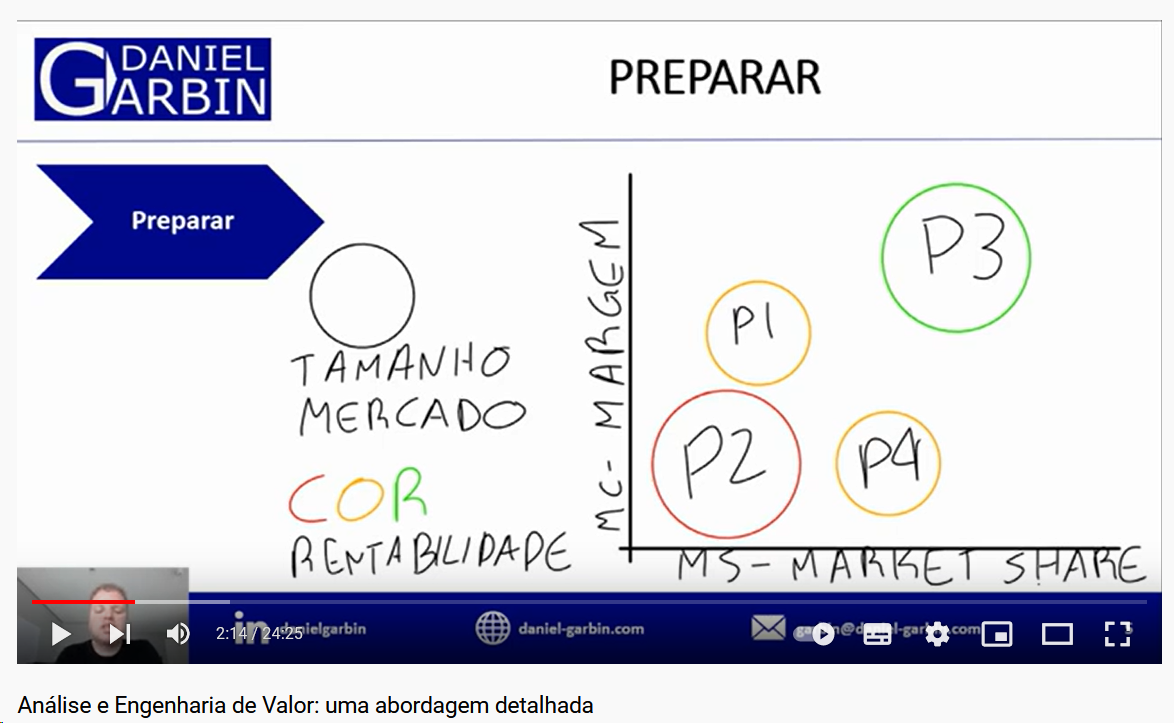
\includegraphics[width=\textwidth]{figures/productSelection.png}
	\end{center}
\end{figure}

It was clear to me that this graph has not just two, but four dimensions: contribution margin (represented by the y-axis), market share (represented by the x-axis), market size (represented by the size of the circle), and profitability ( represented by the color of the circle). \\

In this way then the dimensions of our universe can be understood. \\

I believe that we can experience at least eight dimensions of our universe: width, height and depth, time, shades of red, yellow and blue, and light intensity. \\

Perhaps it is possible in this way to think in other dimensions.

\end{document}
